\documentclass[12pt,]{article}
\usepackage{lmodern}
\usepackage{amssymb,amsmath}
\usepackage{ifxetex,ifluatex}
\usepackage{fixltx2e} % provides \textsubscript
\ifnum 0\ifxetex 1\fi\ifluatex 1\fi=0 % if pdftex
  \usepackage[T1]{fontenc}
  \usepackage[utf8]{inputenc}
\else % if luatex or xelatex
  \ifxetex
    \usepackage{mathspec}
  \else
    \usepackage{fontspec}
  \fi
  \defaultfontfeatures{Ligatures=TeX,Scale=MatchLowercase}
    \setmainfont[]{Times New Roman}
\fi
% use upquote if available, for straight quotes in verbatim environments
\IfFileExists{upquote.sty}{\usepackage{upquote}}{}
% use microtype if available
\IfFileExists{microtype.sty}{%
\usepackage{microtype}
\UseMicrotypeSet[protrusion]{basicmath} % disable protrusion for tt fonts
}{}
\usepackage[margin=2.54cm]{geometry}
\usepackage{hyperref}
\hypersetup{unicode=true,
            pdftitle={Analysis of factors impacting fish and coral abundance across management zones on the inshore coral reefs of the Great Barrier Reef Marine Park},
            pdfauthor={Claire Mullaney},
            pdfborder={0 0 0},
            breaklinks=true}
\urlstyle{same}  % don't use monospace font for urls
\usepackage{color}
\usepackage{fancyvrb}
\newcommand{\VerbBar}{|}
\newcommand{\VERB}{\Verb[commandchars=\\\{\}]}
\DefineVerbatimEnvironment{Highlighting}{Verbatim}{commandchars=\\\{\}}
% Add ',fontsize=\small' for more characters per line
\usepackage{framed}
\definecolor{shadecolor}{RGB}{248,248,248}
\newenvironment{Shaded}{\begin{snugshade}}{\end{snugshade}}
\newcommand{\AlertTok}[1]{\textcolor[rgb]{0.94,0.16,0.16}{#1}}
\newcommand{\AnnotationTok}[1]{\textcolor[rgb]{0.56,0.35,0.01}{\textbf{\textit{#1}}}}
\newcommand{\AttributeTok}[1]{\textcolor[rgb]{0.77,0.63,0.00}{#1}}
\newcommand{\BaseNTok}[1]{\textcolor[rgb]{0.00,0.00,0.81}{#1}}
\newcommand{\BuiltInTok}[1]{#1}
\newcommand{\CharTok}[1]{\textcolor[rgb]{0.31,0.60,0.02}{#1}}
\newcommand{\CommentTok}[1]{\textcolor[rgb]{0.56,0.35,0.01}{\textit{#1}}}
\newcommand{\CommentVarTok}[1]{\textcolor[rgb]{0.56,0.35,0.01}{\textbf{\textit{#1}}}}
\newcommand{\ConstantTok}[1]{\textcolor[rgb]{0.00,0.00,0.00}{#1}}
\newcommand{\ControlFlowTok}[1]{\textcolor[rgb]{0.13,0.29,0.53}{\textbf{#1}}}
\newcommand{\DataTypeTok}[1]{\textcolor[rgb]{0.13,0.29,0.53}{#1}}
\newcommand{\DecValTok}[1]{\textcolor[rgb]{0.00,0.00,0.81}{#1}}
\newcommand{\DocumentationTok}[1]{\textcolor[rgb]{0.56,0.35,0.01}{\textbf{\textit{#1}}}}
\newcommand{\ErrorTok}[1]{\textcolor[rgb]{0.64,0.00,0.00}{\textbf{#1}}}
\newcommand{\ExtensionTok}[1]{#1}
\newcommand{\FloatTok}[1]{\textcolor[rgb]{0.00,0.00,0.81}{#1}}
\newcommand{\FunctionTok}[1]{\textcolor[rgb]{0.00,0.00,0.00}{#1}}
\newcommand{\ImportTok}[1]{#1}
\newcommand{\InformationTok}[1]{\textcolor[rgb]{0.56,0.35,0.01}{\textbf{\textit{#1}}}}
\newcommand{\KeywordTok}[1]{\textcolor[rgb]{0.13,0.29,0.53}{\textbf{#1}}}
\newcommand{\NormalTok}[1]{#1}
\newcommand{\OperatorTok}[1]{\textcolor[rgb]{0.81,0.36,0.00}{\textbf{#1}}}
\newcommand{\OtherTok}[1]{\textcolor[rgb]{0.56,0.35,0.01}{#1}}
\newcommand{\PreprocessorTok}[1]{\textcolor[rgb]{0.56,0.35,0.01}{\textit{#1}}}
\newcommand{\RegionMarkerTok}[1]{#1}
\newcommand{\SpecialCharTok}[1]{\textcolor[rgb]{0.00,0.00,0.00}{#1}}
\newcommand{\SpecialStringTok}[1]{\textcolor[rgb]{0.31,0.60,0.02}{#1}}
\newcommand{\StringTok}[1]{\textcolor[rgb]{0.31,0.60,0.02}{#1}}
\newcommand{\VariableTok}[1]{\textcolor[rgb]{0.00,0.00,0.00}{#1}}
\newcommand{\VerbatimStringTok}[1]{\textcolor[rgb]{0.31,0.60,0.02}{#1}}
\newcommand{\WarningTok}[1]{\textcolor[rgb]{0.56,0.35,0.01}{\textbf{\textit{#1}}}}
\usepackage{graphicx,grffile}
\makeatletter
\def\maxwidth{\ifdim\Gin@nat@width>\linewidth\linewidth\else\Gin@nat@width\fi}
\def\maxheight{\ifdim\Gin@nat@height>\textheight\textheight\else\Gin@nat@height\fi}
\makeatother
% Scale images if necessary, so that they will not overflow the page
% margins by default, and it is still possible to overwrite the defaults
% using explicit options in \includegraphics[width, height, ...]{}
\setkeys{Gin}{width=\maxwidth,height=\maxheight,keepaspectratio}
\IfFileExists{parskip.sty}{%
\usepackage{parskip}
}{% else
\setlength{\parindent}{0pt}
\setlength{\parskip}{6pt plus 2pt minus 1pt}
}
\setlength{\emergencystretch}{3em}  % prevent overfull lines
\providecommand{\tightlist}{%
  \setlength{\itemsep}{0pt}\setlength{\parskip}{0pt}}
\setcounter{secnumdepth}{5}
% Redefines (sub)paragraphs to behave more like sections
\ifx\paragraph\undefined\else
\let\oldparagraph\paragraph
\renewcommand{\paragraph}[1]{\oldparagraph{#1}\mbox{}}
\fi
\ifx\subparagraph\undefined\else
\let\oldsubparagraph\subparagraph
\renewcommand{\subparagraph}[1]{\oldsubparagraph{#1}\mbox{}}
\fi

%%% Use protect on footnotes to avoid problems with footnotes in titles
\let\rmarkdownfootnote\footnote%
\def\footnote{\protect\rmarkdownfootnote}

%%% Change title format to be more compact
\usepackage{titling}

% Create subtitle command for use in maketitle
\providecommand{\subtitle}[1]{
  \posttitle{
    \begin{center}\large#1\end{center}
    }
}

\setlength{\droptitle}{-2em}

  \title{Analysis of factors impacting fish and coral abundance across management
zones on the inshore coral reefs of the Great Barrier Reef Marine Park}
    \pretitle{\vspace{\droptitle}\centering\huge}
  \posttitle{\par}
  \subtitle{\url{https://github.com/cmullane94/ENV_872_Project}}
  \author{Claire Mullaney}
    \preauthor{\centering\large\emph}
  \postauthor{\par}
    \date{}
    \predate{}\postdate{}
  

\begin{document}
\maketitle

\newpage
\tableofcontents 
\newpage
\listoftables 
\newpage
\listoffigures 
\newpage

\hypertarget{rationale-and-research-questions}{%
\section{Rationale and Research
Questions}\label{rationale-and-research-questions}}

Write 1-2 paragraph(s) detailing the rationale for your study. This
should include both the context of the topic as well as a rationale for
your choice of dataset (reason for location, variables, etc.). You may
choose to include citations if you like (optional).

At the end of your rationale, introduce a numbered list of your
questions (or an overarching question and sub-questions).

• Contains clear context for research topic • Contains rationale for
dataset of choice • Contains one or more questions of an appropriate
scope for the project

As the demand for seafood products has increased over the last six
decades, unsustainable fishing, which can result from both illegal
fishing practices as well as poor fisheries management, has been
increasingly recognized as a pressing problem (FAO 2018). Coral reef
fisheries are especially subject to unsustainability because of
increasing coastal populations and the expansion of markets for live
coral reef fishes (Pauly et al.~2002; Bellwood et al.~2004). Reef fish
overexploitation affects the reef community as a whole -- for example,
the targeting of large, predatory reef fish at high trophic levels can
alter and destablize the structure of reef communities (Pauly et
al.~2002; Bellwood et al.~2004; Newton et al.~2007). The negative
effects of overfishing on reef ecosystems -- along with other coral
stressors such as climate change, ocean acidification, and nutrient
pollution -- continue to impact fish communities through the
deterioration of coral, the domination of macroalgae, and decreases in
reef structural complexity (Bellwood et al.~2004; Darling et al.~2017).

The use of no-take marine reserves to conserve reef communities and
manage fishing impacts has increased over the last two decades and have
shown to be effective tools that are capable of increasing fish density,
fish species richness, and coral abundance and health (Williamson et
al.~2004; Lester et al.~2009; Castro-Sanguino et al.~2017). Australia's
Great Barrier Reef is the largest coral reef system in the world, and,
like other reefs worldwide, is exhibiting signs of system-wide
degradation (Bellwood et al.~2004; Fraser et al.~2017). Zoning was first
introduced into the Great Barrier Reef Marine Park (GBRMP) between
1981-1988, and a new zoning management plan was implemented in 2004
(Williamson et al.~2004; Castro-Sanguino et al.~2017).

To examine the effects of GBRMP zoning practices on fish density, fish
species richness, and coral abundance, as well as to determine what
variables impact fish density and coral abundance, a dataset with
varibles concerning zones, fish and coral abundance, and the abundance
of specific fish functional groups was selected -- the chosen dataset is
one of the few projects established with the goal of specifically
assessing the ecological effects of multiple-use zoning on the inshore
coral reefs of the GBRMP (Lawrey 2014). Choice of dataset was also
influenced by timespan -- this project is the only long-term monitoring
project with a dataset that was established prior to the implementation
of the new zoning management plan in 2004 (Lawrey 2014).

This project sought to answer the following questions about the inshore
coral reefs of the GBRMP:

\begin{enumerate}
\def\labelenumi{\arabic{enumi}.}
\tightlist
\item
  What coral reef characterisitics and factors affect the percentage
  cover of live hard coral?
\item
  What coral reef characterisitics and factors affect fish density?
\item
  Do no-take zones established in 1987, no-take zones established in
  2004, and fished zones have different mean amounts of live hard coral
  cover, fish density, and fish species richness?
\end{enumerate}

\newpage

\hypertarget{dataset-information}{%
\section{Dataset Information}\label{dataset-information}}

• Describes source and content of data • Details the wrangling process
from raw to processed data • Contains a table summarizing the dataset
structure

\newpage

\hypertarget{exploratory-analysis}{%
\section{Exploratory Analysis}\label{exploratory-analysis}}

• Flow between text and visualizations is cohesive • Relevant
exploratory information is visualized

\newpage

\hypertarget{analysis}{%
\section{Analysis}\label{analysis}}

• Flow between text and visualizations is cohesive • Visualizations and
statistical tests pertain directly to specific questions • Statistical
results are reported in plain language with relevant statistical output
in parentheses • Findings are reported clearly in relation to research
questions

Insert visualizations and text describing your main analyses. Format
your R chunks so that graphs are displayed but code and other output is
not displayed. Instead, describe the results of any statistical tests in
the main text (e.g., ``Variable x was significantly different among y
groups (ANOVA; df = 300, F = 5.55, p \textless{} 0.0001)''). Each
paragraph, accompanied by one or more visualizations, should describe
the major findings and how they relate to the question and hypotheses.
Divide this section into subsections, one for each research question.

Each figure should be accompanied by a caption, and each figure should
be referenced within the text.

\hypertarget{question-1-what-variables-affect-the-percentage-cover-of-live-hard-coral-on-the-inshore-coral-reefs-of-the-gbrmp}{%
\subsection{Question 1: What variables affect the percentage cover of
live hard coral on the inshore coral reefs of the
GBRMP?}\label{question-1-what-variables-affect-the-percentage-cover-of-live-hard-coral-on-the-inshore-coral-reefs-of-the-gbrmp}}

To determine factors influencing live hard coral cover within the GBRMP,
a mixed-effects analysis of covariance (ANCOVA) model was used. To
account for the random effects of study site and allow extrapolation of
results to potential study sites not included in the data, site was
included as a random effect. The best-fitting model, which was found
using stepwise Akaike information criterion (AIC) analysis, contained
the explanatory variables of year, the mean number of grazer fish
species, the mean number of corallivore fish species, and the mean
percentage cover of fleshy macroalgae. Year, the mean number of grazer
fish species, the mean percentage cover of fleshy macroalgae
significantly decrease the mean percentage of live hard coral cover,
while the mean number of corallivore fish species significantly increase
the mean percentage of live hard coral cover (pseudo
R\textsuperscript{2} = 0.8078; Figures\ldots{}). When all other
variables are held constant, each additional fish included in the mean
number of grazers will decrease mean live hard coral percent cover by
0.0227\% (df = 358, t = -2.805, p \textless{} 0.05). Similarly, a one
unit increase in the mean macroalgae percent cover will decrease mean
live hard coral percent cover by 0.354\% (df = 358, t = 7.641, p
\textless{} 0.0001), while a one unit increase in the mean number of
corallivores will increase mean live hard coral percent cover by 0.265\%
(df = 358, t = 7.812, p \textless{} 0.0001). A post hoc Tukey test was
used to evaluate pairwise relationships of different years and extract
groupings based on these pairwise relationships (Figures\ldots{}).

\begin{figure}

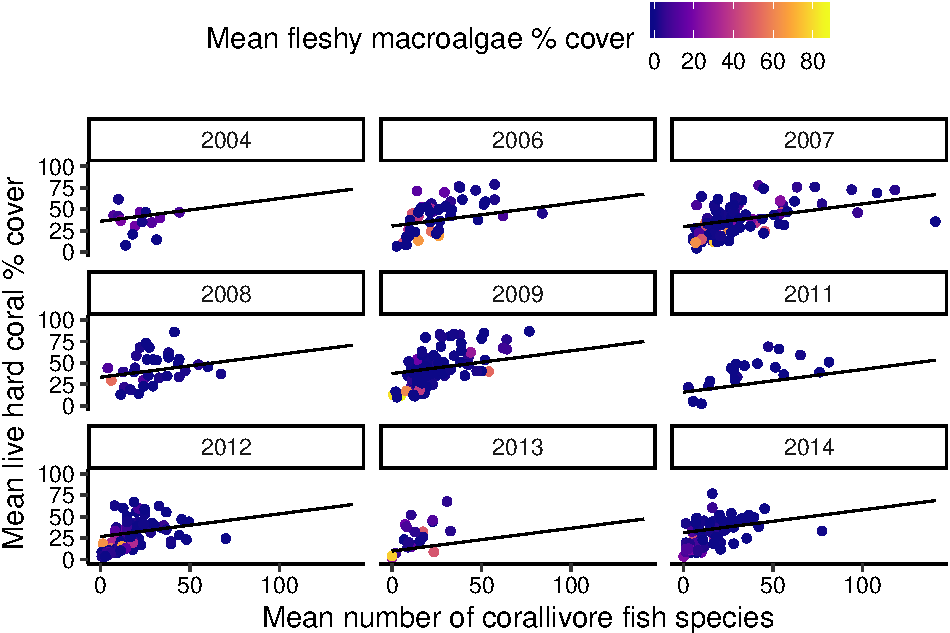
\includegraphics{Mullaney_ENV872_Project_files/figure-latex/Coral Percent Cover Plot (Corallivores)-1} \hfill{}

\caption{Modeled relationship between the mean number of corallivore fish species, the mean percent cover of living hard coral, and the mean percent cover of fleshy macroalgae for 2004, 2006-2009, and 2011-2014. The mean number of grazer fish species was also included in the model (Figure ).Regression lines are plotted using using the mean number of grazer species and the mean percent cover of fleshy macroalgae for the year corresponding to the facet.}\label{fig:Coral Percent Cover Plot (Corallivores)}
\end{figure}

\begin{figure}

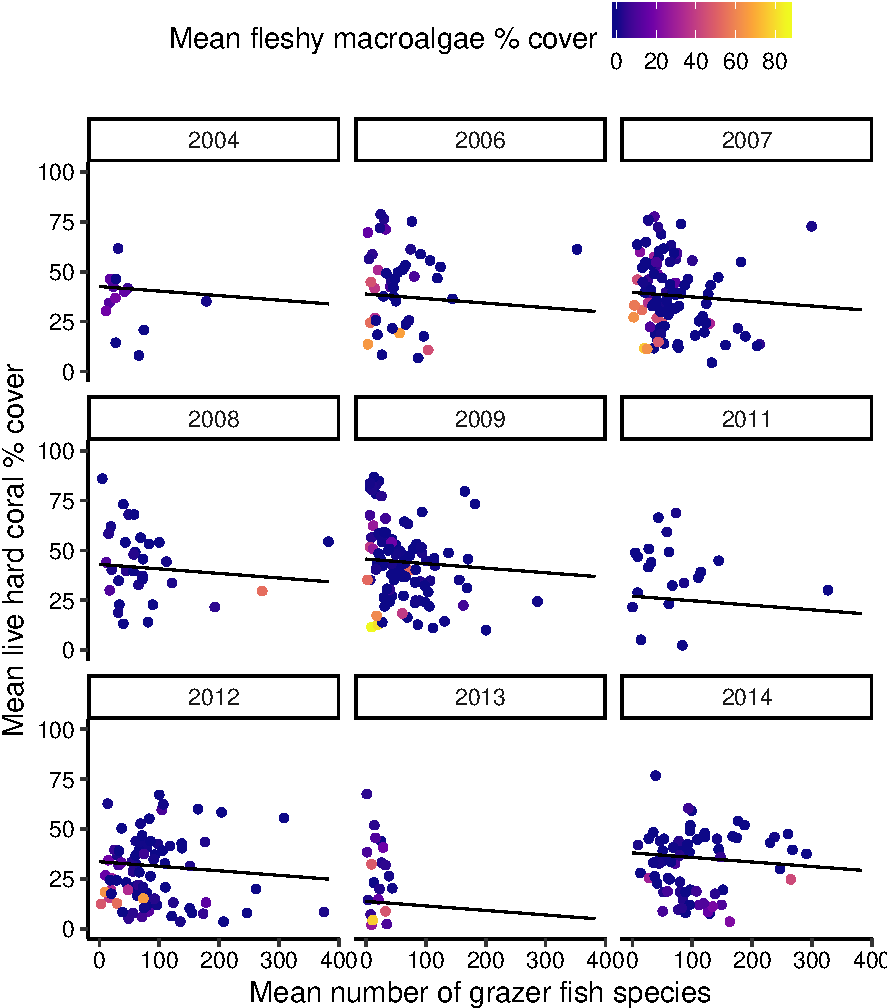
\includegraphics{Mullaney_ENV872_Project_files/figure-latex/Coral Percent Cover Plot (Grazers)-1} \hfill{}

\caption{Modeled relationship between the mean number of grazer fish species, the mean percent cover of living hard coral, and the mean percent cover of fleshy macroalgae for 2004, 2006-2009, and 2011-2014. The mean number of corallivore fish species was also included in the model (Figure ). Regression lines are plotted using using the mean number of corallivore species and the mean percent cover of fleshy macroalgae for the year corresponding to the facet.}\label{fig:Coral Percent Cover Plot (Grazers)}
\end{figure}

\hypertarget{question-2-what-variables-affect-fish-density-on-the-inshore-coral-reefs-of-the-gbrmp}{%
\subsection{Question 2: What variables affect fish density on the
inshore coral reefs of the
GBRMP?}\label{question-2-what-variables-affect-fish-density-on-the-inshore-coral-reefs-of-the-gbrmp}}

To determine factors influencing mean total fish density within the
GBRMP, a mixed-effects analysis of covariance (ANCOVA) model was used.
To again account for the random effects of study site and allow
extrapolation of results to potential study sites not included in the
data, site was included as a random effect. The best-fitting model,
which was found using stepwise AIC analysis, contained the explanatory
variables of year and mean percentage of live hard coral cover. The mean
percentage of live hard coral cover was found to increase the natural
log of mean total fish density (pseudo R\textsuperscript{2} = 0.8087;
Figure\ldots{}). When all other variables are held constant, each
additional 1\% of live hard coral cover will increase the mean total
fish density by 1.536\% (df = 360, t = 7.429, p \textless{} 0.0001). A
post hoc Tukey test was used to evaluate pairwise relationships of
different years and extract groupings based on these pairwise
relationships (Figure\ldots{}).

\begin{figure}

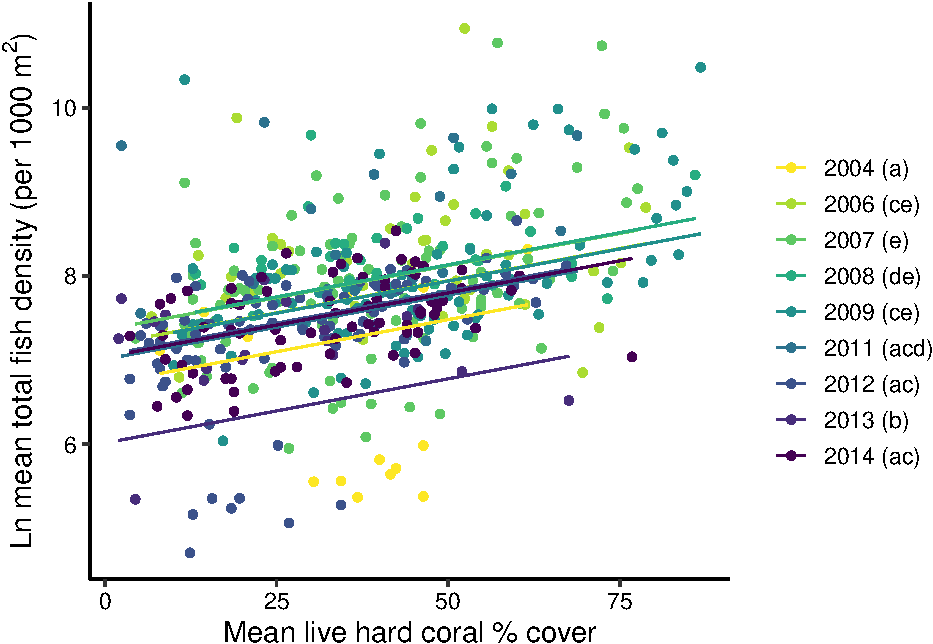
\includegraphics{Mullaney_ENV872_Project_files/figure-latex/Fish Density Plot-1} \hfill{}

\caption{Modeled relationship between the mean percent cover of living hard coral and the natural log of fish density for 2004, 2006-2009, and 2011-2014.}\label{fig:Fish Density Plot}
\end{figure}

\hypertarget{question-3-do-no-take-zones-established-in-1987-no-take-zones-established-in-2004-and-fished-zones-have-different-mean-amounts-of-live-hard-coral-cover-fish-density-and-fish-species-richness}{%
\subsection{Question 3: Do no-take zones established in 1987, no-take
zones established in 2004, and fished zones have different mean amounts
of live hard coral cover, fish density, and fish species
richness?}\label{question-3-do-no-take-zones-established-in-1987-no-take-zones-established-in-2004-and-fished-zones-have-different-mean-amounts-of-live-hard-coral-cover-fish-density-and-fish-species-richness}}

\begin{Shaded}
\begin{Highlighting}[]
\CommentTok{#LHC}
\NormalTok{LHC_zone_plot <-}\StringTok{ }\KeywordTok{ggplot}\NormalTok{(GBR_Sites_Processed_}\DecValTok{1999}\NormalTok{) }\OperatorTok{+}
\StringTok{  }\KeywordTok{aes}\NormalTok{(}\DataTypeTok{x =}\NormalTok{ Zone, }\DataTypeTok{y =}\NormalTok{ LHC_mean) }\OperatorTok{+}
\StringTok{  }\KeywordTok{geom_boxplot}\NormalTok{() }\OperatorTok{+}
\StringTok{  }\KeywordTok{stat_summary}\NormalTok{(}\DataTypeTok{geom =} \StringTok{"text"}\NormalTok{, }\DataTypeTok{fun.y =}\NormalTok{ max, }\DataTypeTok{vjust =} \DecValTok{-1}\NormalTok{, }\DataTypeTok{size =} \FloatTok{3.5}\NormalTok{,}
               \DataTypeTok{label =} \KeywordTok{c}\NormalTok{(}\StringTok{"a"}\NormalTok{, }\StringTok{"a"}\NormalTok{, }\StringTok{"a"}\NormalTok{)) }\OperatorTok{+}
\StringTok{  }\KeywordTok{ylim}\NormalTok{(}\DecValTok{0}\NormalTok{, }\DecValTok{100}\NormalTok{) }\OperatorTok{+}
\StringTok{  }\KeywordTok{labs}\NormalTok{(}\DataTypeTok{y =} \StringTok{"Mean live hard coral % cover"}\NormalTok{) }\OperatorTok{+}
\StringTok{  }\KeywordTok{theme}\NormalTok{(}\DataTypeTok{axis.title.y =} \KeywordTok{element_text}\NormalTok{(}\DataTypeTok{size =} \DecValTok{10}\NormalTok{))}

\CommentTok{#Fish density}
\NormalTok{Fish_densit_zone_plot <-}\StringTok{ }\KeywordTok{ggplot}\NormalTok{(GBR_Sites_Processed_}\DecValTok{2004}\NormalTok{) }\OperatorTok{+}
\StringTok{  }\KeywordTok{aes}\NormalTok{(}\DataTypeTok{x =}\NormalTok{ Zone, }\DataTypeTok{y =} \KeywordTok{log}\NormalTok{(Total.Fish.Densit_mean)) }\OperatorTok{+}
\StringTok{  }\KeywordTok{geom_boxplot}\NormalTok{() }\OperatorTok{+}
\StringTok{  }\KeywordTok{stat_summary}\NormalTok{(}\DataTypeTok{geom =} \StringTok{"text"}\NormalTok{, }\DataTypeTok{fun.y =}\NormalTok{ max, }\DataTypeTok{vjust =} \DecValTok{-1}\NormalTok{, }\DataTypeTok{size =} \FloatTok{3.5}\NormalTok{,}
               \DataTypeTok{label =} \KeywordTok{c}\NormalTok{(}\StringTok{"b"}\NormalTok{, }\StringTok{"b"}\NormalTok{, }\StringTok{"a"}\NormalTok{)) }\OperatorTok{+}
\StringTok{  }\KeywordTok{ylim}\NormalTok{(}\FloatTok{4.5}\NormalTok{, }\DecValTok{11}\NormalTok{) }\OperatorTok{+}
\StringTok{  }\KeywordTok{labs}\NormalTok{(}\DataTypeTok{y =} \KeywordTok{expression}\NormalTok{(}\StringTok{'Ln mean total fish density (per 1000 m'}\OperatorTok{^}\StringTok{"2"}\OperatorTok{*}\StringTok{')'}\NormalTok{)) }\OperatorTok{+}
\StringTok{  }\KeywordTok{theme}\NormalTok{(}\DataTypeTok{axis.title.x =} \KeywordTok{element_blank}\NormalTok{(), }\DataTypeTok{axis.text.x =} \KeywordTok{element_blank}\NormalTok{(),}
        \DataTypeTok{axis.title.y =} \KeywordTok{element_text}\NormalTok{(}\DataTypeTok{size =} \DecValTok{10}\NormalTok{))}

\CommentTok{#Fish species richness}
\NormalTok{Fish_species_rich_plot <-}\StringTok{ }\KeywordTok{ggplot}\NormalTok{(GBR_Sites_Processed_}\DecValTok{2004}\NormalTok{) }\OperatorTok{+}
\StringTok{  }\KeywordTok{aes}\NormalTok{(}\DataTypeTok{x =}\NormalTok{ Zone, }\DataTypeTok{y =}\NormalTok{ Fish.Species.richness_mean) }\OperatorTok{+}
\StringTok{  }\KeywordTok{geom_boxplot}\NormalTok{() }\OperatorTok{+}
\StringTok{  }\KeywordTok{stat_summary}\NormalTok{(}\DataTypeTok{geom =} \StringTok{"text"}\NormalTok{, }\DataTypeTok{fun.y =}\NormalTok{ max, }\DataTypeTok{vjust =} \DecValTok{-1}\NormalTok{, }\DataTypeTok{size =} \FloatTok{3.5}\NormalTok{,}
               \DataTypeTok{label =} \KeywordTok{c}\NormalTok{(}\StringTok{"a"}\NormalTok{, }\StringTok{"a"}\NormalTok{, }\StringTok{"a"}\NormalTok{)) }\OperatorTok{+}
\StringTok{  }\KeywordTok{ylim}\NormalTok{(}\DecValTok{5}\NormalTok{, }\DecValTok{51}\NormalTok{) }\OperatorTok{+}
\StringTok{  }\KeywordTok{labs}\NormalTok{(}\DataTypeTok{y =} \StringTok{"Mean number of fish species observed"}\NormalTok{) }\OperatorTok{+}
\StringTok{  }\KeywordTok{theme}\NormalTok{(}\DataTypeTok{axis.title.x =} \KeywordTok{element_blank}\NormalTok{(), }\DataTypeTok{axis.text.x =} \KeywordTok{element_blank}\NormalTok{(),}
              \DataTypeTok{axis.title.y =} \KeywordTok{element_text}\NormalTok{(}\DataTypeTok{size =} \DecValTok{10}\NormalTok{))}

\CommentTok{#Plotting all three graphs in one plot}
\KeywordTok{plot_grid}\NormalTok{(Fish_species_rich_plot, Fish_densit_zone_plot, LHC_zone_plot, }\DataTypeTok{ncol =} \DecValTok{1}\NormalTok{)}
\end{Highlighting}
\end{Shaded}

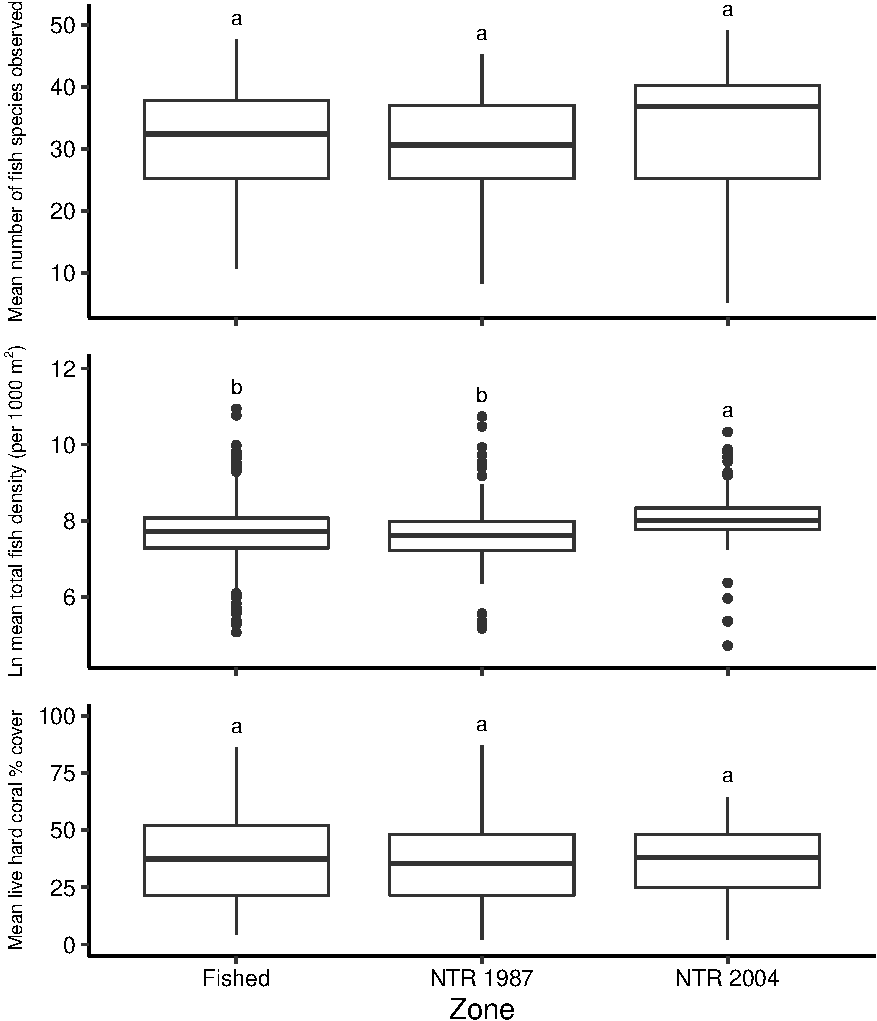
\includegraphics{Mullaney_ENV872_Project_files/figure-latex/Zoning Plots-1.pdf}
\newpage

\hypertarget{summary-and-conclusions}{%
\section{Summary and Conclusions}\label{summary-and-conclusions}}

• Major findings are summarized • Conclusions relate back to the
original research context

\newpage

\hypertarget{references}{%
\section{References}\label{references}}

Bellwood DR, Hughes TP, Folke C, Nyström M. 2004. Confronting the coral
reef crisis. Nature. 429(6994):827--833. \url{doi:10.1038/nature02691}.

Castro-Sanguino C, Bozec Y-M, Dempsey A, Samaniego BR, Lubarsky K,
Andrews S, Komyakova V, Ortiz JC, Robbins WD, Renaud PG, et al.~2017.
Detecting conservation benefits of marine reserves on remote reefs of
the northern GBR. PLoS ONE. 12(11):e0186146.

Darling ES, Graham NA, J, Januchowski-hartley FA, Nash KL, Pratchett MS,
Wilson SK. 2017. Relationships between structural complexity, coral
traits, and reef fish assemblages. Coral Reefs; Heidelberg.
36(2):561--575. \url{doi:http://dx.doi.org/10.1007/s00338-017-1539-z}.

FAO, editor. 2018. Meeting the sustainable development goals. Rome (The
state of world fisheries and aquaculture).

Fraser KA, Adams VM, Pressey RL, Pandolfi JM. 2017. Purpose, policy, and
practice: Intent and reality for on-ground management and outcomes of
the Great Barrier Reef Marine Park. Marine Policy. 81:301--311.
\url{doi:10.1016/j.marpol.2017.03.039}.

Lawrey E. 2014. e-Atlas Dataset reporting form.

Lester SE, Halpern BS, Grorud-Colvert K, Lubchenco J, Ruttenberg BI,
Gaines SD, Airamé S, Warner RR. 2009. Biological effects within no-take
marine reserves: a global synthesis. Marine Ecology Progress Series.
384:33--46. \url{doi:10.3354/meps08029}.

Newton K, Côté IM, Pilling GM, Jennings S, Dulvy NK. 2007. Current and
Future Sustainability of Island Coral Reef Fisheries. Current Biology.
17(7):655--658. \url{doi:10.1016/j.cub.2007.02.054}.

Pauly D, Christensen V, Guénette S, Pitcher TJ, Sumaila UR, Walters CJ,
Watson R, Zeller D. 2002. Towards sustainability in world fisheries.
Nature. 418(6898):689--695. \url{doi:10.1038/nature01017}.

Williamson DH, Russ GR, Ayling AM. 2004. No-take marine reserves
increase abundance and biomass of reef fish on inshore fringing reefs of
the Great Barrier Reef. Environmental Conservation. 31(2):149--159.
\url{doi:10.1017/S0376892904001262}.


\end{document}
